\subsection{過去の点$x$を参照にして次の点を選択する場合}

1の場合には、$X_{i}$を選ぶ確率とそのうえで$x$が選ばれる確率は独立であるというものであった。しかし、これまで考えたように、単にそのようなモデルを考えただけだと$X_{i}$の数$N$の効果をうまく反映できないように思える。したがって、次に考えるモデルは前に選ばれた点に近い点が選ばれることにし、そのときその点をもつ$X_{i}$が選ばれたとするモデルである。

$X_{i}$はそれぞれ$s_{i}$個の点をもっており、モデルの設定時に仮定したとおり、これらの点は異なる$X$同士で共有されることはない。はじめに点$x_{0}$が与えられ、次に時刻$1$では、それぞれの$X$の中で最もその点に近いものを選び、より近いものをもった$X$の順に整列する。この$X$の順番にしたがって、$X_{i}$にそれぞれに割り当てられた確率$P_{i}$で、実際にその点$x$が選択されるかどうかが決定する。点が選択されない場合(確率$1-P_{i}$)ときは、$X$の順番で次の順番になっているものについて、同様の試行を繰り返す。もしすべての$X$について点$x$が選択されないときは、時刻$k$を一つすすめ、その時刻には$x_{0}$が選ばれたとする。
\begin{figure}[H]
    \begin{center}
        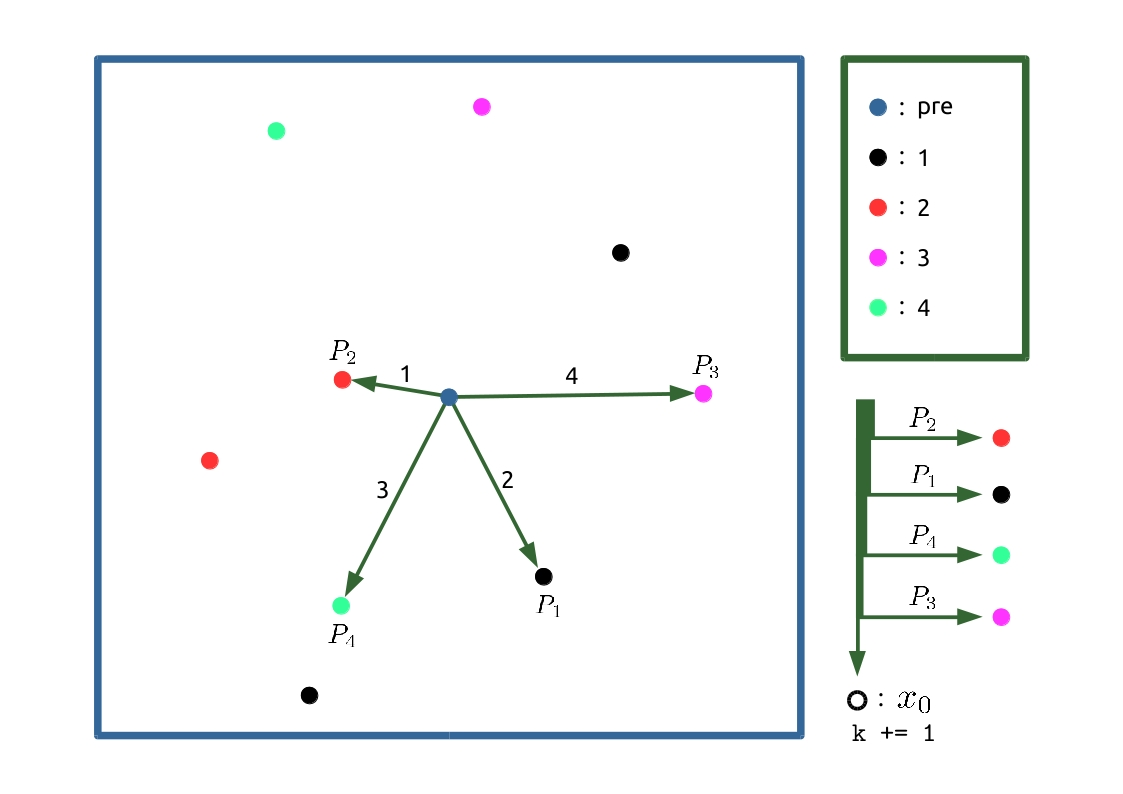
\includegraphics[width=12.5cm]{../img/figure2.jpg}
        \caption{$[0,1]$の数直線上で閾値$r$で定められる領域}
        \label{fig:f8}
    \end{center}
\end{figure}

図\ref{fig:f8}を用いて説明する。中心にある"pre"と名のついた点が参照する一つの点であり、この次の時刻に選ばれる点の選び方は、まずそれぞれの$X_{i}$について"pre"に最も近い点を選び、その近さの順に順番を付けることにする。図で青枠内の緑の矢印に示された数字がそれぞれの$X_{i}$の順番である。この順番にしたがってそれぞれの$X_{i}$に割り当てられた$P_{i}$にしたがって実際にその点が選ばれるかどうかが決まる。右下の矢印はそのことを表したフローチャートになっている。すべての$X_{i}$について点が選ばれなかった場合、時刻を一つ進め、はじめの点$x_{0}$を選択する。

参照する点の選び方として、以下のような場合分けを考えた。

\begin{enumerate}
    \item なし (case 1)
    \item 一つの点
    \begin{enumerate}
        \item 時刻0における点 (case 2)
        \item 一つ前の時刻の点 (case 3)
        \end{enumerate}
    \item 二つの点
    \begin{enumerate}
        \item 時刻0における点 + 一つ前の時刻の点 (case 4)
        \item 二つ前の時刻までの点 (case 5)
        \end{enumerate}
\end{enumerate}

\subsubsection{過去の点の影響を受けない場合 (case 1)}

$X_{i}$が$X$の配列の中で$r+1$($r = 1, 2, \cdots , n-1$)番目に選ばれたとき、$X_{i}$まで順番が回ってくる確率は
$$p_{r+1}(i) = \frac{\sum_{J = \langle j_{0}, \cdots ,j_{r-1} \rangle _{r}}\prod_{j\in J}(1-P_{j})}{_{n-1}C_{r}}.$$
ここで$J = \langle j_{0}, j_{1}, \cdots ,j_{r-1} \rangle_{r}$は、$i$を除く$n-1$個の要素から$r$個選んだときの組み合わせのうちの1揃いをあらわすことにする。

また、1番目に$x$を選択する権利を得たときに、選択権が回ってくる確率は当然
$$p_{1}(i) = 1$$
である。

説明のための具体的な例として、$N = 5, n = 5, i = 1, r = 2$とすると、$X_{1}$までに2つの$X$が選択権を得ているはずであり、その2つの組み合わせは$(0,2), (0,3), (0,4), (2,3), (2,4), (3,4)$の6つの組み合わせがある。上の式では$J$の一つは$(0, 2)$であり、このとき$j_{0} = 0, j_{1} = 2$である。この$J$に関して和をとり、組み合わせの数$\ _{4}C_{2} = 6$で割って期待値を求めている。
\begin{align}
p_{r+1}(1) &= \left[(1-P_{0})(1-P_{2}) + (1-P_{0})(1-P_{3}) + (1-P_{0})(1-P_{4}) \right. \nonumber \\
&\ \left. + (1-P_{2})(1-P_{3}) + (1-P_{2})(1-P_{4}) + (1-P_{3})(1-P_{4}) \right]/6
\end{align}
$X_{i}$が選択権の順番で$r$番目になる確率は等しいので、$r$に関する平均をとり、$P_{i}$をかければ、これは$X_{i}$から点が選ばれる確率の期待値となる。

$$p(i) = \frac{\sum_{r=0}^{n}p_{r}(i)P_{i}}{n}.$$

このとき得られた確率は$X_{i}$によって異なり、期待値としては毎時刻ごとにそれぞれの$X_{i}$がその確率が点が選択されることになり、単純な確率過程に帰着できる。

